\section{Mixture of Experts (MoE)}
\begin{frame}{}
    \LARGE \textbf{Mixture of Experts (MoE)}
\end{frame}

\begin{frame}[allowframebreaks]{MoE Overview}
    \begin{figure}
        \centering
        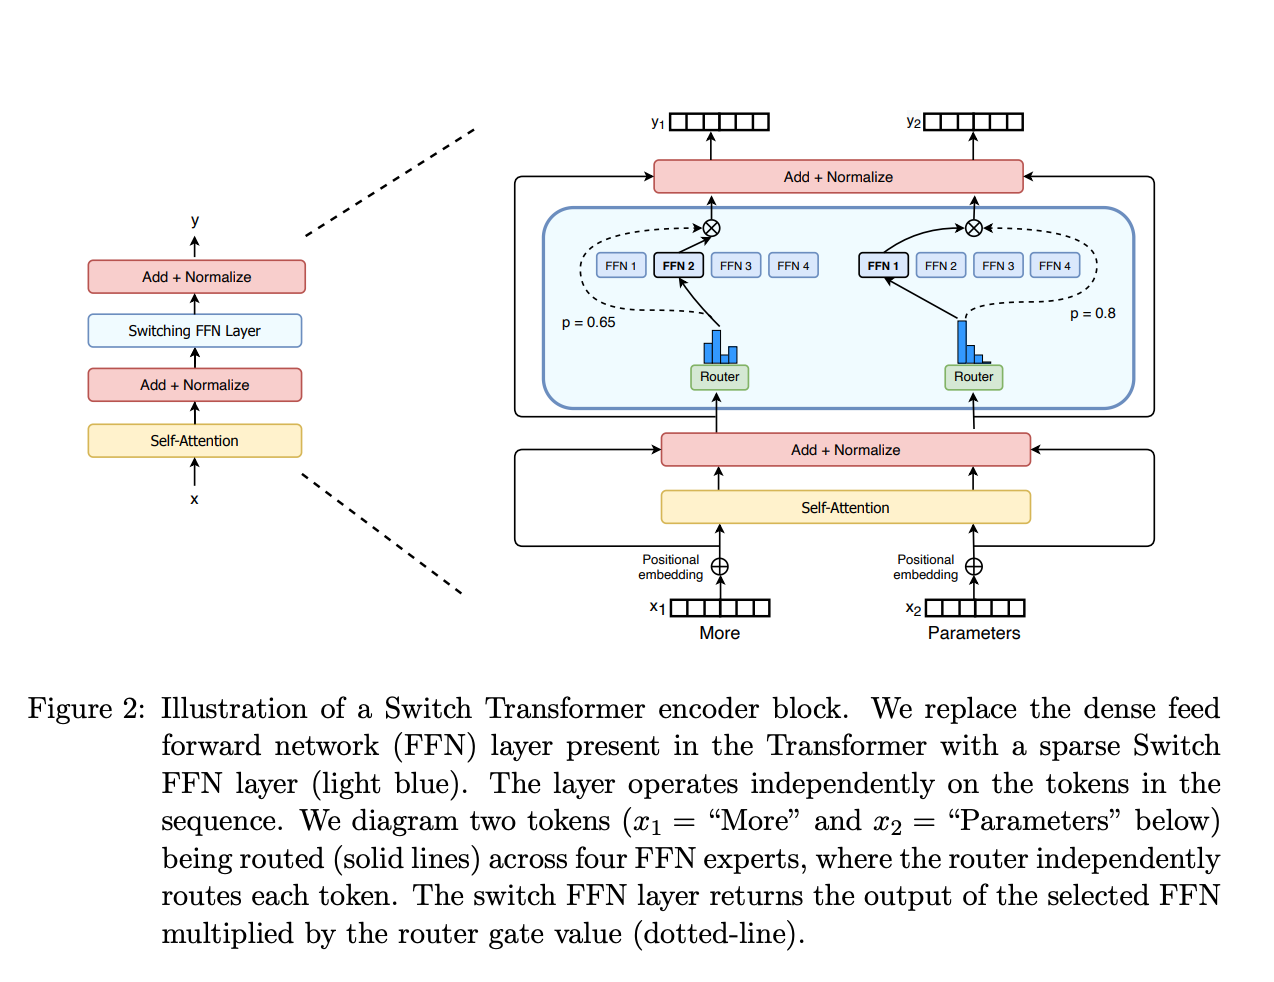
\includegraphics[height=0.9\textheight,width=1\textwidth,keepaspectratio]{images/recent-advance/moe-switch-transformer.png}
    \end{figure}
\framebreak

    \textbf{Mixture of Experts (MoE)} is a neural network architecture that uses multiple "expert" subnetworks to process inputs, allowing for efficient scaling and specialization.

    \begin{itemize}
        \item \textbf{Experts:} Each expert is a small neural network trained on specific tasks or data.
        \item \textbf{Gating Mechanism:} A gating network decides which experts to activate for each input, enabling dynamic routing.
        \item \textbf{Scalability:} MoE models can scale to billions of parameters while maintaining computational efficiency.
    \end{itemize}
\end{frame}

\begin{frame}{MoE: Key Idea}
    \begin{itemize}
        \item \textbf{Key Idea:} Activate only a subset of the model for each input, rather than the entire network.
        \item Each input is routed to a small number of experts (typically 2 out of N), improving efficiency.
        \item A gating network determines which experts are selected for each input.
    \end{itemize}
\end{frame}

\begin{frame}{Notable MoE Papers}
    \begin{itemize}
        \item Switch Transformer (Fedus et al., 2021): Efficient routing and scaling.
        \item GShard (Lepikhin et al., 2020): Large-scale MoE for multilingual translation.
        \item M6, GLaM, and recent GPT-MoE variants: Further advances in scaling and performance.
    \end{itemize}
\end{frame}

\begin{frame}[allowframebreaks]{What is Sparsity?}
    \begin{itemize}
        \item \textbf{Sparsity:} Refers to the condition where only a small fraction of the model's parameters are active at any given time.
        \item In MoE, sparsity is achieved by activating only a few experts for each input, leading to reduced computational cost.
        \item This allows for larger models without a proportional increase in computation.
    \end{itemize}

\framebreak

    \begin{itemize}
        \item \textbf{Gating Network:} Learns to route inputs to experts. Output is:
        \[
            y = \sum_{i=1}^{n} G(x)_i E_i(x)
        \]
        \item \textbf{Sparsity:} If $G(x)_i = 0$, expert $E_i$ is skipped, saving compute.
        \item \textbf{Typical Gating:} Softmax over a linear projection:
        \[
            G_\sigma(x) = \text{Softmax}(x W_g)
        \]
        \item \textbf{Noisy Top-k Gating:} Adds noise for load balancing, selects top $k$ experts:
        \[
            H(x)_i = (x W_g)_i + \text{StandardNormal()} \cdot \text{Softplus}((x W_{noise})_i)
        \]
        \[
            G(x) = \text{Softmax}(\text{KeepTopK}(H(x), k))
        \]
        \item \textbf{Benefits:} Activating few experts speeds up training/inference and improves load balancing.
    \end{itemize}
\end{frame}

\begin{frame}[allowframebreaks]{Load Balancing in MoEs}
    \textbf{Problem:} Without intervention, the gating network tends to route most tokens to a few experts, leading to inefficient training and poor expert utilization.

    \begin{itemize}
        \item \textbf{Expert Overload:} Popular experts receive more tokens, train faster, and become even more favored.
        \item \textbf{Underutilization:} Other experts receive few or no tokens, limiting their contribution.
    \end{itemize}

    \textbf{Solution:} Introduce an auxiliary loss to encourage balanced token distribution across experts.

    \begin{itemize}
        \item \textbf{Auxiliary Loss:} Penalizes uneven assignment of tokens, pushing the gating network to distribute tokens more uniformly.
        \item \textbf{Expert Capacity:} Each expert is assigned a maximum number of tokens it can process (capacity). Excess tokens are dropped or rerouted.
        \item \textbf{Implementation:} In transformer-based MoEs, this is often controlled via an \texttt{aux\_loss} parameter.
    \end{itemize}

    \textbf{Auxiliary Loss Example:}
    \[
        L_{\text{aux}} = n \cdot \sum_{i=1}^{n} f_i \log f_i
    \]
    where $f_i$ is the fraction of tokens assigned to expert $i$, and $n$ is the number of experts.

    \textbf{Benefits:}
    \begin{itemize}
        \item Ensures all experts are trained and utilized.
        \item Improves model efficiency and generalization.
        \item Prevents bottlenecks and overload in popular experts.
    \end{itemize}
\end{frame}

\begin{frame}[allowframebreaks]{MoEs and Transformers}
    \textbf{Transformers and Scaling:} Transformers demonstrate that increasing the number of parameters improves performance. Google’s GShard project explored scaling transformers beyond 600 billion parameters using MoE layers.

    \begin{itemize}
        \item \textbf{GShard Approach:} Replaces every other feed-forward (FFN) layer with an MoE layer using top-2 gating in both encoder and decoder.
        \item \textbf{Distributed Training:} MoE layers are shared across devices, while other layers are replicated, enabling efficient large-scale computation.
    \end{itemize}

    \begin{figure}
        \centering
        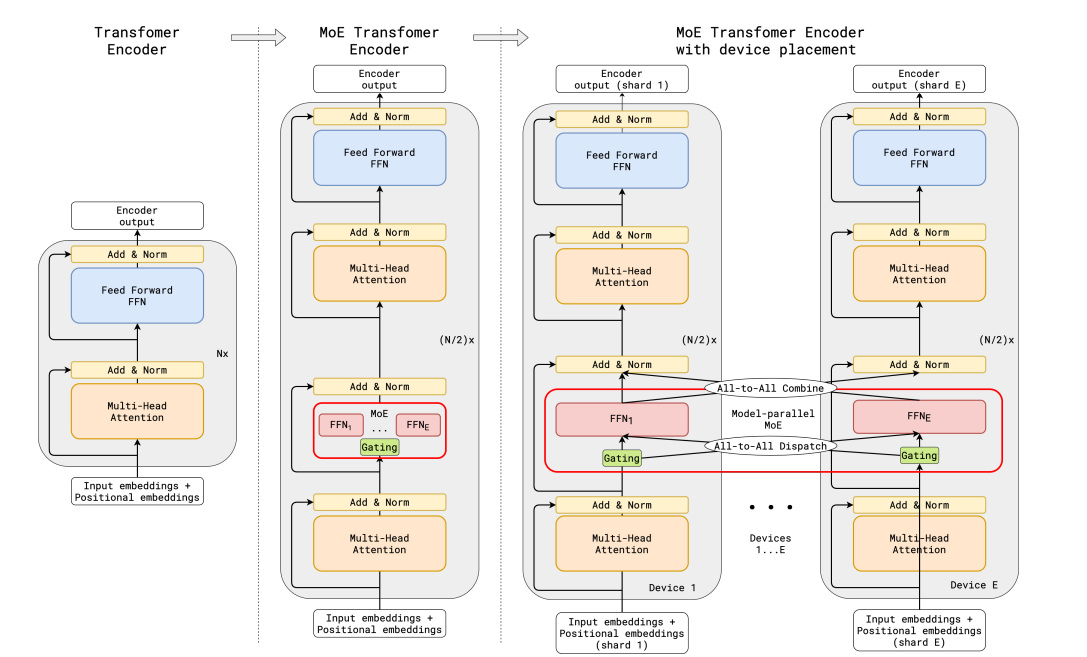
\includegraphics[height=0.8\textheight,width=1\textwidth,keepaspectratio]{images/recent-advance/gshard-moe-encoder.png}
        \caption*{MoE Transformer Encoder from the GShard Paper}
    \end{figure}

\framebreak

    \textbf{Load Balancing and Efficiency:}
    \begin{itemize}
        \item \textbf{Random Routing:} In top-2 gating, the top expert is always selected, while the second expert is chosen probabilistically based on its gating weight.
        \item \textbf{Expert Capacity:} Each expert has a maximum token capacity. Overflow tokens are either sent via residual connections or dropped, ensuring static tensor shapes and balanced computation.
    \end{itemize}

    \textbf{Why Expert Capacity?}
    \begin{itemize}
        \item Tensor shapes must be fixed at compile time, but token distribution to experts is dynamic. Capacity factors ensure compatibility and efficiency.
    \end{itemize}

\framebreak

    \textbf{Inference Efficiency:}
    \begin{itemize}
        \item During inference, only a subset of experts is activated per input.
        \item Shared computations (e.g., self-attention) are applied to all tokens, so the effective compute is much lower than the total parameter count.
        \item Example: A 47B parameter model with 8 experts can run with the compute of a 12B dense model; with top-2 gating, 14B parameters are used.
    \end{itemize}
\end{frame}

\begin{frame}[allowframebreaks]{Switch Transformers}
    \textbf{Switch Transformers:} Address training and fine-tuning instabilities in MoEs by simplifying routing and improving efficiency. The authors released a 1.6T parameter MoE model with 2048 experts on Hugging Face, achieving a 4x pre-train speed-up over T5-XXL.

    \begin{itemize}
        \item \textbf{Switch Transformer Layer:} Replaces FFN layers with MoE layers, but routes each token to a single expert (single-expert strategy), reducing router computation and communication costs while preserving quality.
        \item \textbf{Expert Capacity:} Defined as
        \[
            \text{Expert Capacity} = \left(\frac{\text{tokens per batch}}{\text{number of experts}}\right) \times \text{capacity factor}
        \]
        \item Low capacity factors (1--1.25) are effective, balancing efficiency and communication overhead.
        \item \textbf{Load Balancing Loss:} Simplified auxiliary loss encourages uniform routing and is weighted by a hyperparameter.
        \item \textbf{Selective Precision:} Experts are trained in bfloat16, while routing uses full precision to avoid instability. This reduces communication and computation costs without degrading quality.
    \end{itemize}

\framebreak

    \begin{figure}
        \centering
        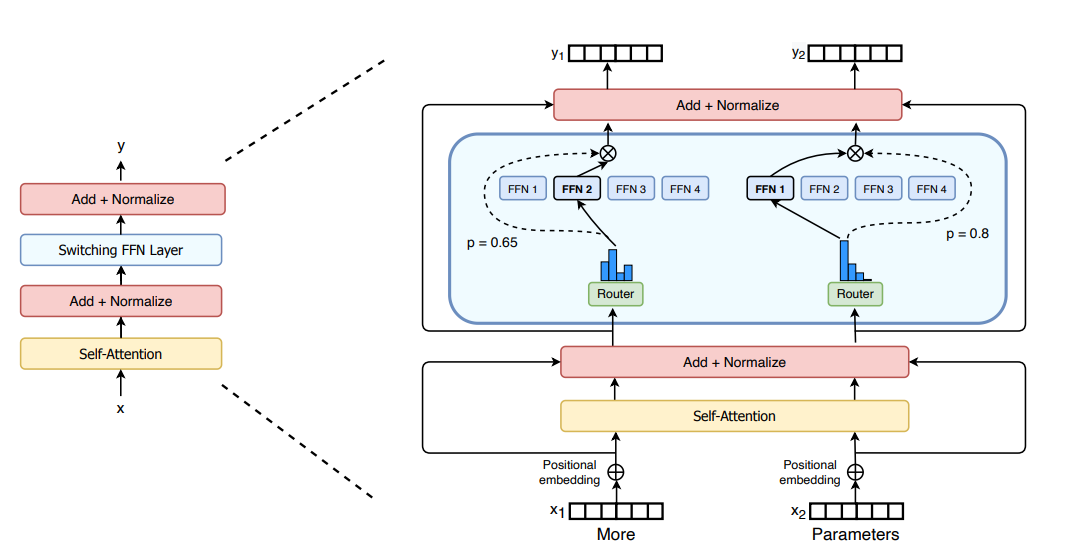
\includegraphics[height=0.9\textheight,width=1\textwidth,keepaspectratio]{images/recent-advance/moe-switch-trans.png}
    \end{figure}

\framebreak

    \textbf{Architecture:}
    \begin{itemize}
        \item Encoder-decoder setup, similar to T5 but with MoE layers.
        \item Fine-tuning and summarization tasks are supported.
    \end{itemize}

    \textbf{GLaM and Scaling:}
    \begin{itemize}
        \item GLaM explores scaling MoEs further, matching GPT-3 quality with 1/3 the energy.
        \item Uses decoder-only models, top-2 routing, and larger capacity factors.
        \item Capacity factor can be adjusted during training and inference to control compute and efficiency.
    \end{itemize}
\end{frame}

\begin{frame}{Sparse MoEs vs Dense Models}
    \textbf{When to Use Sparse MoEs:}
    \begin{itemize}
        \item Ideal for high-throughput scenarios with access to many machines.
        \item Given a fixed compute budget for pretraining, sparse MoEs are more optimal due to efficient parameter utilization.
        \item Enables scaling to very large models without a proportional increase in computation.
    \end{itemize}

    \textbf{When to Use Dense Models:}
    \begin{itemize}
        \item Preferable for low-throughput scenarios or when limited VRAM is available.
        \item Simpler to implement and deploy on single devices.
        \item More suitable for smaller-scale tasks or resource-constrained environments.
    \end{itemize}

    \textbf{Note:} The number of parameters in sparse and dense models cannot be directly compared, as they represent fundamentally different architectures and computational trade-offs.
\end{frame}

\begin{frame}[allowframebreaks]{Parallelism in MoE}
    \textbf{Parallelism Overview:}
    \begin{itemize}
        \item \textbf{Data Parallelism:} Replicates model weights across all cores; data is partitioned so each core processes a different batch.
        \item \textbf{Model Parallelism:} Splits the model across cores; each core holds a part of the model, and data is replicated.
        \item \textbf{Model and Data Parallelism:} Both model and data are partitioned; different cores process different batches and hold different model segments.
        \item \textbf{Expert Parallelism:} Experts are distributed across workers. Each worker processes a different batch, and MoE layers route tokens to the appropriate expert on each worker.
    \end{itemize}

    \textbf{Expert Parallelism Details:}
    \begin{itemize}
        \item For non-MoE layers, expert parallelism acts like data parallelism.
        \item For MoE layers, tokens are dynamically routed to the worker hosting the selected expert.
        \item Enables scaling to large numbers of experts and efficient distributed training.
    \end{itemize}

    \begin{figure}
        \centering
        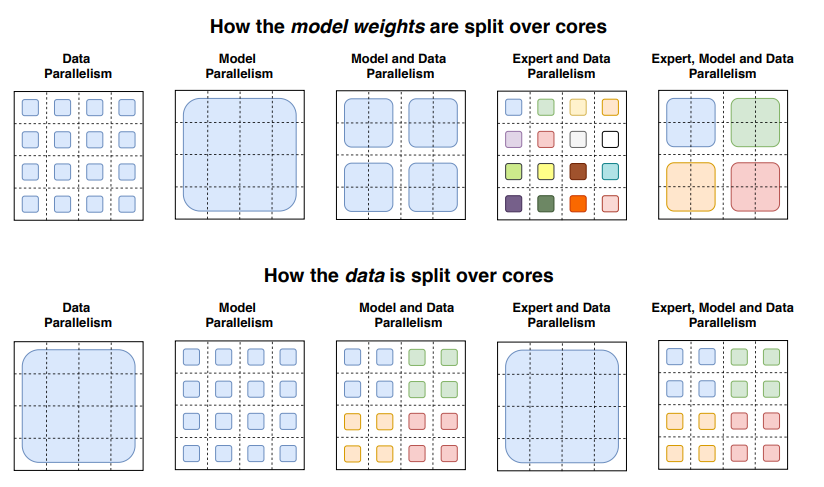
\includegraphics[height=0.6\textheight,width=1\textwidth,keepaspectratio]{images/recent-advance/moe-parallelism.png}
        \caption*{Illustration of model, expert, and data parallelism (adapted from Switch Transformers)}
    \end{figure}
\end{frame}

\begin{frame}[allowframebreaks]{Transformer vs. Mixture of Experts in LLMs}
    \textbf{Dense Transformers:}
    \begin{itemize}
        \item Every input token passes through all layers and all parameters.
        \item Simpler architecture and easier to implement.
        \item Scaling up increases both parameter count and computational cost proportionally.
        \item Well-suited for moderate-scale models and resource-constrained environments.
    \end{itemize}

\framebreak

    \textbf{Mixture of Experts (MoE):}
    \begin{itemize}
        \item Only a subset of experts (subnetworks) are activated for each input.
        \item Enables scaling to massive parameter counts without proportional increase in compute.
        \item Requires gating networks and load balancing mechanisms.
        \item More complex to implement and train, but highly efficient for large-scale distributed training.
    \end{itemize}

\framebreak

    \begin{figure}
        \centering
        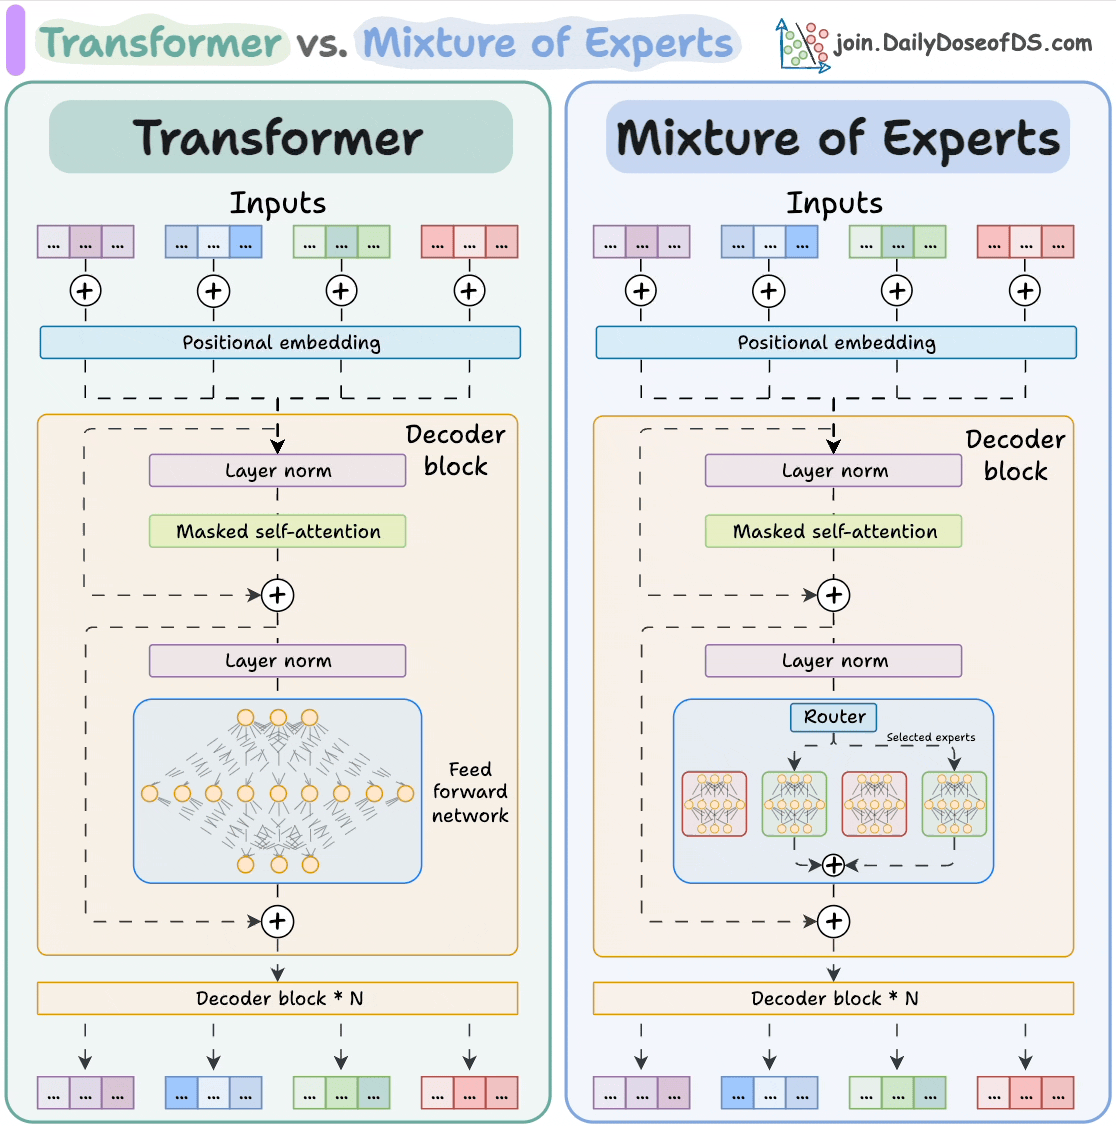
\includegraphics[height=0.9\textheight,width=1\textwidth,keepaspectratio]{images/recent-advance/moe-transformer.png}
    \end{figure}

\framebreak

    \textbf{Comparison:}
    \begin{itemize}
        \item \textbf{Efficiency:} MoEs are more compute-efficient for large models, as only a fraction of parameters are used per token.
        \item \textbf{Scalability:} MoEs allow scaling to trillions of parameters, while dense transformers are limited by hardware constraints.
        \item \textbf{Specialization:} MoEs can specialize experts for different data or tasks, potentially improving performance.
        \item \textbf{Complexity:} Dense transformers are easier to deploy and maintain; MoEs require careful engineering for routing and load balancing.
    \end{itemize}

\framebreak

    \textbf{Use Cases:}
    \begin{itemize}
        \item Dense transformers: Small to medium LLMs, single-device inference, low-latency applications.
        \item MoEs: Large-scale pretraining, multi-device distributed systems, scenarios where efficiency and specialization are critical.
    \end{itemize}
\end{frame}

\begin{frame}{MoE: Advantages}
    \begin{itemize}
        \item Scales efficiently to very large models.
        \item Reduces computation cost per token by activating only a few experts.
        \item Well-suited for distributed training across multiple devices.
        \item Enables specialization among experts, potentially improving performance.
    \end{itemize}
\end{frame}

\begin{frame}{MoE: Challenges}
    \begin{itemize}
        \item Complex routing and expert selection mechanisms.
        \item Load balancing: Ensuring all experts are utilized effectively.
        \item Training instability and convergence issues.
        \item Increased implementation complexity compared to standard models.
    \end{itemize}
\end{frame}